\documentclass[aspectratio=169]{beamer}
\usetheme{default}
\usepackage{amsmath,amssymb,tikz}
\setbeamertemplate{navigation symbols}{}
\title{Principal Component Analysis}
\subtitle{Lecture 7 -- Unsupervised Learning}
\date{}
\begin{document}

\frame{\titlepage}

\begin{frame}{Motivation}
\begin{itemize}
  \item Data often lives in high dimension: images, gene expression, sensor arrays
  \item But most variation happens along a few directions
  \item Goal: find a low-dimensional linear subspace that keeps most of the variance
  \item Uses: visualisation, compression, denoising, preprocessing for regression
\end{itemize}
\end{frame}

\begin{frame}{Setup}
\begin{itemize}
  \item Data matrix $X \in \mathbb{R}^{n \times d}$, rows $x_i$, centred: $\frac1n\sum_i x_i = 0$
  \item Sample covariance $S = \frac{1}{n} X^\top X$
  \item Project onto a unit vector $w$: $z_i = w^\top x_i$
  \item Variance of the projection: $\operatorname{Var}(z) = w^\top S w$
\end{itemize}
\end{frame}

\begin{frame}{First principal component}
\[
  w_1 = \arg\max_{\|w\|=1} w^\top S w
\]
\begin{itemize}
  \item Lagrangian: $w^\top S w - \lambda (w^\top w - 1)$
  \item Stationarity: $S w = \lambda w$ \quad $\Rightarrow$ $w$ is an eigenvector of $S$
  \item Variance captured $= \lambda$ \quad $\Rightarrow$ take the \textbf{largest} eigenvalue
\end{itemize}
\end{frame}

\begin{frame}{Geometric picture}
\centering
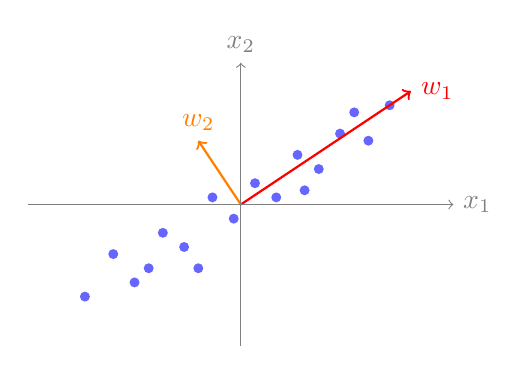
\begin{tikzpicture}[scale=0.9]
  \foreach \x/\y in {-2.2/-1.3,-1.8/-0.7,-1.5/-1.1,-1.1/-0.4,-0.8/-0.6,-0.4/0.1,-0.1/-0.2,0.2/0.3,
                     0.5/0.1,0.8/0.7,1.1/0.5,1.4/1.0,1.8/0.9,2.1/1.4,-0.6/-0.9,0.9/0.2,1.6/1.3,-1.3/-0.9}
    \fill[blue!60] (\x,\y) circle (2pt);
  \draw[->,thick,red] (0,0) -- (2.4,1.6) node[right] {$w_1$};
  \draw[->,thick,orange] (0,0) -- (-0.6,0.9) node[above] {$w_2$};
  \draw[gray,->] (-3,0) -- (3,0) node[right] {$x_1$};
  \draw[gray,->] (0,-2) -- (0,2) node[above] {$x_2$};
\end{tikzpicture}

\small $w_1$ points along the direction of largest spread, $w_2 \perp w_1$
\end{frame}

\begin{frame}{$k$ components and explained variance}
\begin{itemize}
  \item Eigendecomposition $S = V \Lambda V^\top$, $\lambda_1 \ge \lambda_2 \ge \dots \ge \lambda_d \ge 0$
  \item Keep the top $k$ eigenvectors $W_k = [w_1,\dots,w_k]$, scores $Z = X W_k$
  \item Explained variance ratio: $\dfrac{\sum_{j\le k}\lambda_j}{\sum_{j\le d}\lambda_j}$
  \item Choose $k$ from a scree plot or a threshold (e.g.\ 95\%)
\end{itemize}
\end{frame}

\begin{frame}{Computing PCA with the SVD}
\begin{itemize}
  \item Thin SVD of the centred data: $X = U \Sigma V^\top$
  \item Then $S = \frac1n V \Sigma^2 V^\top$: right singular vectors = principal directions
  \item Eigenvalues $\lambda_j = \sigma_j^2 / n$
  \item Numerically stabler than forming $X^\top X$; cost $O(n d \min(n,d))$
\end{itemize}
\end{frame}

\begin{frame}{Reconstruction view}
\begin{itemize}
  \item Reconstruction from $k$ components: $\hat x_i = W_k W_k^\top x_i$
  \item PCA minimises the mean squared reconstruction error among all rank-$k$ projections
  \item Error $= \sum_{j>k} \lambda_j$ (the discarded variance)
\end{itemize}
\end{frame}

\begin{frame}{Pitfalls}
\begin{itemize}
  \item Always centre the data; standardise features with different units
  \item PCA is linear: curved manifolds need kernel PCA or autoencoders
  \item Sensitive to outliers (variance is a squared quantity)
  \item Components maximise variance, not class separation (compare LDA)
\end{itemize}
\end{frame}

\end{document}
